\NeedsTeXFormat{LaTeX2e}[1995/12/01]
\documentclass[10pt]{bmcart}
%\documentclass[twocolumn]{bmcart}% uncomment this for twocolumn layout and comment line below
%%% additional documentclass options:
%  [doublespacing]
%  [linenumbers]   - put the line numbers on margins

% Load packages
\usepackage{url}  % Formatting web addresses  
\urlstyle{rm}
\usepackage[utf8]{inputenc} %unicode support
\usepackage{amssymb}
%\usepackage{cite}
\usepackage{graphicx}
\usepackage{multirow}
 
%%%%%%%%%%%%%%%%%%%%%%%%%%%%%%%%%%%%%%%%%%%%%%%%%	
%%                                             %%
%%  If you wish to display your graphics for   %%
%%  your own use using includegraphic or       %%
%%  includegraphics, then comment out the      %%
%%  following two lines of code.               %%   
%%  NB: These line *must* be included when     %%
%%  submitting to BMC.                         %% 
%%  All figure files must be submitted as      %%
%%  separate graphics through the BMC          %%
%%  submission process, not included in the    %% 
%%  submitted article.                         %% 
%%                                             %%
%%%%%%%%%%%%%%%%%%%%%%%%%%%%%%%%%%%%%%%%%%%%%%%%%                     

%\def\includegraphic{}
%\def\includegraphics{}

%%% Put your definitions there:
\startlocaldefs
\endlocaldefs


%%%%%%%%%%%%%%%%%%%%%%%%%%%% RESEARCH PAPER %%%%%%%%%%%%%%%%%%%%%%%%%%%%%%%%%%%

\begin{document}

%%% Start of article front matter
\begin{frontmatter}

\begin{fmbox}
\dochead{Research}

\title{The Chemistry Development Kit (CDK). 3. Atom typing, Rendering, Molecular Formula, and Substructure Searching}

% FIXME: finish migrating the author list

\author[
   addressref={um},                   % id's of addresses, e.g. {aff1,aff2}
   %corref={aff1},                       % id of corresponding address, if any
   %noteref={n1},                        % id's of article notes, if any
   email={egon.willighagen@maastrichtuniversity.nl}   % email address
]{\inits{ELW}\fnm{Egon L} \snm{Willighagen}}
\author[
   addressref={aff2},
   email={john@nextmovesoftware.com}
]{\inits{JWM}\fnm{John W} \snm{May}}
\author[
   addressref={uppsala},
   email={jonathan.alvarsson@farmbio.uu.se}
]{\inits{JA}\fnm{Jonathan} \snm{Alvarsson}}
\author[
   addressref={uppsala},
   email={berg.arvid@gmail.com}
]{\inits{AB}\fnm{Arvid} \snm{Berg}}
\author[
   addressref={jena},
   email={kai.duehrkop@uni-jena.de}
]{\inits{KD}\fnm{Kai} \snm{Dührkop}}
\author[
   addressref={idea},
   email={jeliazkova.nina@gmail.com}
]{\inits{NJ}\fnm{Nina} \snm{Jeliazkova}}
\author[
   addressref={wi_mit},
   email={pluskal@wi.mit.edu}
]{\inits{TP}\fnm{Tomáš}~\snm{Pluskal}}
\author[
   addressref={???},
   email={miguelrojasch@googlemail.com}
]{\inits{MRJ}\fnm{Miguel}~\snm{Rojas-Cherto}}
\author[
   addressref={uppsala},
   email={ola.spjuth@farmbio.uu.se}
]{\inits{OS}\fnm{Ola} \snm{Spjuth}}
\author[
   addressref={???},
   email={gilleain.torrance@gmail.com}
]{\inits{GT}\fnm{Gilleain} \snm{Torrance}}
\author[
   addressref={um},
   email={chris.evelo@maastrichtuniversity.nl}
]{\inits{CTE}\fnm{Chris T} \snm{Evelo}}
\author[
   addressref={nih},
   email={guhar@mail.nih.gov}
]{\inits{RG}\fnm{Rajarshi} \snm{Guha}}
\author[
   addressref={ebi},
   email={steinbeck@ebi.ac.uk}
]{\inits{CS}\fnm{Christoph}~\snm{Steinbeck}}

\address[id=um]{
  \orgname{Dept of Bioinformatics - BiGCaT, NUTRIM, Maastricht University}, % university, etc
  %\street{Waterloo Road},                     %
  \postcode{NL-6200 MD},
  \city{Maastricht},                              % city
  \cny{The Netherlands}                                    % country
}
\address[id=aff2]{
  \orgname{??},
  %\street{D\"{u}sternbrooker Weg 20},
  %\postcode{24105},
  %\city{Kiel},
  \cny{UK}
}
\address[id=uppsala]{
  \orgname{Department of Pharmaceutical Biosciences, Uppsala University},
  %\street{D\"{u}sternbrooker Weg 20},
  \postcode{751 24},
  \city{Uppsala},
  \cny{Sweden}
}
\address[id=jena]{
  \orgname{Chair for Bioinformatics, Friedrich Schiller University},
  %\street{},
  \postcode{07743},
  \city{Jena},
  \cny{Germany}
}
\address[id=idea]{
  \orgname{Ideaconsult Ltd},
  \street{A. Kanchev 4},
  \postcode{1000},
  \city{Sofia},
  \cny{Bulgaria}
}
\address[id=wi_mit]{
  \orgname{Whitehead Institute for Biomedical Research}, 
  \street{9 Cambridge Center},
  \postcode{MA 02142},
  \city{Cambridge},
  \cny{USA}
}
\address[id=nih]{
  \orgname{National Center for Advancing Translational Science},
  \street{9800 Medical Center Drive},
  \postcode{MD 20878},
  \city{Rockville},
  \cny{USA}
}
\address[id=ebi]{
  \orgname{Chemoinformatics and Metabolism team, European Bioinformatics Institute},
  %\street{A. Kanchev 4},
  %\postcode{1000},
  \city{Hinxton},
  \cny{UK}
}

%\begin{artnotes}
%\note{Sample of title note}     % note to the article
%\note[id=n1]{Equal contributor} % note, connected to author
%\end{artnotes}

\end{fmbox}% comment this for two column layout

%% The Abstract begins here
\begin{abstractbox}

\begin{abstract}
% Do not use inserted blank lines (ie \\) until main body of text.
\parttitle{Background}
Cheminformatics is a well-established field with many applications in chemistry,
biology, drug discovery, and others. The Chemistry Development Kit (CDK) has
become a widely used Open Source cheminformatics toolkit, providing various models to represent
chemical structures, of which the chemical graph is essential. However,
in the first five years of the project increased so much in size that
interdependencies between components grew unmanageable large, resulting
in unpredictable instabilities.
\parttitle{Results}
We here report improvements to the CDK since the 1.2 release series made
to accommodate both the increased complexity of the library, as well as
significant improvements of and additions to the functionality of the
library. Second, we outline how the CDK evolved with respect to
quality control and the approach we have adopted to ensure stability, including
a peer review mechanism.
Additionally, a selection of the new APIs that have been introduced will
be discussed: atom type perception, substructure searching, molecular
fingerprints, rendering of molecules, and handling of molecular formulas.
\parttitle{Conclusions}
With this paper we have shown the continued effort to provide a free, Open Source
cheminformatics library, and show that such collaborative projects can exist over
a long period. We have taken advantage from the community support, and show
that an open source cheminformatics project can act as a peer reviewed
publishing platform for scientific computing software.
\end{abstract}

\begin{keyword}
\kwd{Java}
\kwd{cheminformatics}
\kwd{bioinformatics}
\end{keyword}

% MSC classifications codes, if any
%\begin{keyword}[class=AMS]
%\kwd[Primary ]{}
%\kwd{}
%\kwd[; secondary ]{}
%\end{keyword}

\end{abstractbox}
%
%\end{fmbox}% uncomment this for twcolumn layout

\end{frontmatter}


%%%%%%%%%%%%%%%%
%% Background %%
%%
\section*{Background}

Open Source cheminformatics has made significant steps forward recently~\cite{OBoyle2011}.
The Chemistry Development Kit (CDK) is one of the tools under the Blue Obelisk wings,
and previously documented version have been widely adopted~\cite{Steinbeck2003,Steinbeck2006}.
For example, new tools expose CDK functionality in larger platforms such as Cinfony~\cite{OBoyle2008},
rcdk~\cite{Guha2007}, and plugins for Taverna~\cite{Truszkowski2011},
KNIME~\cite{Beisken2013}, ChemViz2 for Cytoscape~\cite{ChemViz2}, and LICSS for
Microsoft Excel~\cite{Lawson2012}.
Furthermore, projects with specific functionality have emerged building on the CDK, including
jCompoundMapper~\cite{Hinselmann2011}, ScaffoldHunter~\cite{wetzel2009interactive}, OMG~\cite{Peironcely2012},
Padel~\cite{yap2011padel}, AMBIT-SMARTS~\cite{jeliazkova2011ambitsmarts}, AMBIT-Tautomer~\cite{kochev2013ambit},
ReactPRED~\cite{ReactPRED}, SMSD~\cite{Rahman2009,Rahman2014}, WhichCyp~\cite{Rostkowski2013},
and MetaPrint2D~\cite{Carlsson2010}. Other tools used previous versions already, and follow
newer releases of the CDK, such as Bioclipse~\cite{spjuth2007bioclipse,
spjuth2009bioclipse} and AMBIT~\cite{jeliazkova2011ambit}. While the above
tools suggest that the CDK is primarily used to create general tools, it is
important to note that it is also used to solve specific questions, like finding
the maximally bridging rings in chemical structures~\cite{Marth2015}.

However, previous version of the CDK were written by a community with specific applications
in mind, of which structure elucidation was one. It could therefore be rather competitive
in some cheminformatics domains, such as fingerprinting~\cite{Clark2014,Cannon2006}, in other parts
it could be inadequate, such in the capturing of stereochemistry.

Continued community development of the CDK in the last few years, however, has shown that
Open Source software is here to stay. The adoption of automatic build systems and
quality control methodologies such as unit testing, automated source code validation,
and peer review by fellow developers have greatly improved the stability of the library,
At the expense of slowing down the development, it has allowed for cleaning up interdependencies
between modules of code, and has reset the scalability of the development model,
allowing for a lot of new functionality in code APIs while maintaining the quality
of code depending on those core APIs.

This has resulted in important improved functionality, such as a separately published
InChI functionality~\cite{Spjuth2013} and greatly improved ring detection functionality~\cite{May2014},
but also a core atom type perception module, covering a much wider set of elements than
previous CDK versions and capturing many more charged and radical atom species,
a more comprehensive fingerprinting API, many speed and stability improvements, and more.

%%%%%%%%%%%%%%%%%%%%%%%%%%%%
%% Results and Discussion %%
%%
\section*{Results and Discussion}

\subsection*{New APIs and improved implementations}

We here outline various new and improved APIs in the CDK library since the two previous
publications.

  \subsubsection*{Atom Typing}

  Atom type perception is a core cheminformations functionality: the atom types describe
  chemical features of atoms, such as the number of neighbors, possible formal charges,
  (approximate) hybridization, electron distribution over orbitals, etc. However, the
  CDK commonly integrated atom type perception into algorithms, resulting in multiple
  and diverging copies of similar atom type schemes. With the need to add many
  new atom types for previously uncovered element, but also charged and radical atom
  types, a new approach was needed.
  
  This CDK version has isolated a new atom typing framework, removing the perception of
  atom types from various algorithms, allowing the perception to be tested separately.
  The new code defines the atom types using a list that specifies for each type
  the element symbol, hybridization, formal charge, number of lone pairs, and
  an enumeration of the bond orders (see Figure~1). This list of properties captures the
  information needed for the various algorithms in the CDK. For example,
  hybridization information can be used in certain aromaticity models (see later),
  and the lone pair information is needed for resonance structure calculation
  needed, for example, for Gasteiger $\pi$-charges.

  A reference perception class, CDKAtomTypeMatcher, has been written that perceives these atom types, and
  validates the perception automatically against the properties defined by the ontology.
  This class handles a variety in types of missing information, as commonly resulting
  from various (file) formats; for example, it can handle undefined hydrogen counts
  and undefined double bond positions if hybridization information is provided instead.
  That makes the code complex, and at times slow, but so far shown sufficiently
  performant for many applications. Possibly, in the future
  alternative algorithms may be implemented, while that would again increase the maintenance
  burden.

  \subsubsection*{Stereochemistry}

  In previous versions of the API, stereochemistry was represented disparately hindering 
  interconversion between and within file formats. In CDK 1.5.x the core representation 
  has been standardized upon and procedures updated or added to enable duplicate checking,
  pattern matching, and interconversion.

  The preferred representation of stereochemistry is now for it to be stored at the molecule
  level as a \texttt{\textbf{StereoElement}}. In abstract terms a stereo element describes local
  geometry using a type, focus, carriers, and configuration (Figure~2\ref{fig:stereodatastructure}).
  Currently the most common types of stereochemistry are supported: Tetrahedral, Cis-trans isomerism 
  around a double bond, and Extended Tetrahedral. Rarer types of stereochemistry, such as: Square 
  Planar, Trigonal Bipyramidal, Octahedral, could easily be incorporated into the chosen description 
  given sufficient demand from the community.


  Along with the new stereochemistry representation, algorithms were required in several areas. Generally
  a user does not need to invoked these procedures explicitly as they are called as needed within existing
  APIs:

  \begin{itemize}
   \item perception from 2D coordinates;
   \item perception from 3D coordinates;
   \item wedge assignment;
   \item graph (sub)isomorphism matching;
   \item SMARTS matching; and
   \item canonicalization.
  \end{itemize}

  The perception from coordinates and wedge assignment algorithms are fundamental for conversion
  between formats that store stereochemistry implicitly based on coordinates (e.g. Molfile, CML) and 
  explicitly (e.g. SMILES, CML, InChI). Perception from 2D coordinates can optionally identify
  perspective projects, specifically: Fischer, Haworth, and Chair projections. With the perception of 
  perspective projections enabled, database entries currently consider distinct can be merged
  (Figure~3\ref{fig:stereoprojections}). The perception is based on an algorithm briefly 
  described by \cite{Karapetyan2015}.

  % ChEMBL 21 ~2281 structures (~11454 TH center) drawn in perspective

  Graph matching of stereochemistry with the described representation is straight forward. Given
  the atom-atom mapping from a query structure to a target molecule, the focus and carriers of 
  the query stereochemistry are mapped to the target. Using the permutation parity of this mapping
  the configurations compared. SMARTS matching requires some special handling for complex cases 
  \cite{May2014_SMARTS}. For canonicalization, a partial canonical ordering is used to assign an 
  absolute label which can then be integrated into the ordering. More detailed descriptions of 
  these algorithms are described in detail in Chapter 6 of \cite{May2015}.

  \subsubsection*{Signatures}

  An implementation has been provided of the Signature structure descriptor for
  molecules~\cite{Faulon2003}. These act as a linear notation - like the SMILES format - 
  for the whole molecule as well as for connected substructures rooted at a single atom. The 
  descriptor can also be canonicalized to provide isomorphism-independent
  representations~\cite{Faulon2004}, and has been successfully used in QSAR modeling~\cite{signaturefingerprints,Spjuth2011DS,Moghadam2015,Alvarsson2014,Spjuth2012OS,Norinder2013}.

  \subsubsection*{Rendering API}

  A new rendering API has been introduced to make the rendering code independent
  from Java widget toolkits. The previous code was tightly linked to the Swing
  toolkit, but other tools use different widget toolkits. For example, Bioclipse
  is based on Eclipse which uses the SWT~\cite{spjuth2007bioclipse}. %FIXME: write SWT in full
  
  A second new design goal was introduced to balance between size restrictions
  of some use cases, such as Java applets, and the rendering functionality. In
  particular, some functionality, even after Modularization, needed considerable
  parts of the CDK library, making creation if a small-sized applet unfeasible.
  Therefore, the rendering API was modularized to allow splitting up rendering
  functionality into modules, with varying CDK dependencies.
  
  % DESCRIBE THE CORE APIs
  
  Moreover, a simplified API has been introduced that addresses most of the
  common rendering needs, with the DepictionGenerator class. To depict benzene
  the following code can be used:

\begin{verbatim}
new DepictionGenerator()
  .withSize(300, 300)
  .depict(benzene)
  .writeTo("BenzeneLocalized.png");
\end{verbatim}

  Many of the rendering options are available as parameters in the core API
  and as methods on the DepictionGenerator class. This includes substructure
  coloring, exemplified with this example reaction (see Fig.~2\ref{fig:depiction}):

\begin{verbatim}
TODO
\end{verbatim}

  \subsubsection*{Structure Diagram Layout}

  The structure diagram layout has been rewritten and the new code solves a
  number of long standing issues. Particularly, collision detection has been
  greatly improved. Figure~5\ref{fig:sdg} shows a difference in output between
  the old code base, with and without overlap resolving, and with the new code.
  The new code can be used like:

\begin{verbatim}
TODO
\end{verbatim}

  \subsubsection*{Molecular Formula}

  A chemical formula is the basic/simple chemical representation of a compound.
It defines the number of isotopes or elements that constitute the composition
of a compound without describing how atoms are bonded. With the rise of
metabolomics it has become increasingly relevant to have full support for these
in cheminformatics libraries~\cite{RojasCherto2011}.

  The CDK interfaces can handle several concepts related to chemical formulas:
the formula itself, sets of formulas, chemical formula ranges, adducts, isotope
containers and patterns, and rules to filter formula sets. These new tools can
be used for a number of tasks, including calculating the isotopic pattern from
a given chemical formula, determining the possible elemental compositions for a
given mass (mass decomposition), and calculating the exact mass from a given
chemical formula.

  The CDK contains two algorithms for the decomposition of mass ranges into
possible elemental formulas. For most inputs, a Round Robin algorithm,
originally developed for the SIRIUS metabolite identification
tool~\cite{Bocker2009}, is used. The algorithm discretizes the real-value mass
decomposition problem into an integer-value knapsack
problem~\cite{Martello1990}. It first computes a dynamic programming table and
then backtracks it to generate matching formulas~\cite{Duehrkop2013,
Boecker2008}. Data for the Round Robin algorithm is stored in an extended
residue table~\cite{Bocker2005}, resulting in a low memory footprint of several
kilobytes. For certain problem instances, such as very large mass values (above
$400\,000$ Da) or mass range span larger than $1$ Da, the Round Robin algorithm
is not applicable and CDK falls back to an optimized full enumeration search
method, originally developed as part of the MZmine~2 framework for mass
spectrometry data processing~\cite{Pluskal2012, Pluskal2010}.

  The following code calculates all possible chemical formulas for a given
accurate mass, within allowed counts for each element:

\begin{verbatim}
Isotopes ifac = Isotopes.getInstance();
MolecularFormulaRange range =
  new MolecularFormulaRange();
range.addIsotope( ifac.getMajorIsotope("C"), 8, 20);
range.addIsotope( ifac.getMajorIsotope("H"), 0, 20);
range.addIsotope( ifac.getMajorIsotope("O"), 0, 1);
range.addIsotope( ifac.getMajorIsotope("N"), 0, 1);

MolecularFormulaGenerator tool =
  new MolecularFormulaGenerator(
    SilentChemObjectBuilder.getInstance(),
    133.0, 133.1, range
  );
IMolecularFormulaSet mfSet = tool.getAllFormulas();
for (mf in mfSet) {
  println MolecularFormulaManipulator.getString(mf) + " " +
    MolecularFormulaManipulator.getTotalExactMass(mf)
}
\end{verbatim}

This gives the following output:

\begin{verbatim}
C11H 133.007825032
C9H11N 133.089149352
C9H9O 133.065339908
C8H7NO 133.052763844
\end{verbatim}

   To evaluate the performance of the CDK molecular formula generator, we
compared its runtimes on a range of inputs and compared them to the runtimes of
the classic, full enumeration-based HR2 formula generator~\cite{Kind2007} and
those of a recently developed Parallel Formula Generator (PFG)~\cite{Zhang2016}
(Table~1\ref{tab:formula_generators}). Although for small mass values the PFG
algorithm achieved shorter runtimes, for larger masses the Round Robin
algorithm implemented in CDK clearly outperformed the two other methods.


  \subsubsection*{SMILES parser and generator}

  The SMILES parsing has been replaced code in the external Beam project~\cite{Beam}.
  This BSD-licensed SMILES parser is a complete implementation of the SMILES
  and OpenSMILES (\url{http://opensmiles.org/}) specifications by one of the
  authors (including stereochemistry), and is independent of
  the CDK library. The SmilesParser API uses this library underneath, and the
  Beam API is hidden by this class. The most significant change here is that
  the SMILES parser now automatically locates the positions of double bonds,
  but this can be turned off:

\begin{verbatim}
  SmilesParser parser = new SmilesParser(
    SilentChemObjectBuilder.getInstance()
  );
  parser.kekulise(false);
  mol = parser.parseSmiles(smi);
\end{verbatim}

  The SMILES generation API has also been simplified and made more flexible.
  Creating unique SMILES or aromatic SMILES is now done by first creating a
  SMILES generator instance which can make generic or unique SMILES, and with
  or without simplifying aromatic rings using the lower case element symbols
  for the organic subset. This generator can then be repeatedly called:

\begin{verbatim}
  uniqueGenerator = SmilesGenerator.unique()
  aromaticGenerator = SmilesGenerator.generic().aromatic()
  smiles = uniqueGenerator.createSMILES(mol)
  smiles2 = atomaticGenerator.createSMILES(mol)
\end{verbatim}

  \subsubsection*{Substructure searching}

  TODO: iterator and new SMARTS

  \subsubsection*{Ring finding}

  Ring finding is a key functionality in a cheminformatics library, and the CDK
  knows a long history of ring finding~\cite{May2014}. Particularly, non-redundant
  ring sets have seen particular interest, such as the smallest set of smallest
  rings, for which the CDK implements two classical algorithms~\cite{Figueras1996,Berger2004}.
  Recent work by one the authors has implemented a new, faster algorithm, allowing
  searching for various types of (non-redundant) ring sets~\cite{May2014}. These
  are available via the new Cycles API:

\begin{verbatim}
  allCycles = Cycles.all(mol)
  relevantCycles = Cycles.relevant(mol)
  essentialCycles = Cycles.essential(mol)
  sssrCycles = Cycles.sssr(mol)
\end{verbatim}

  \subsubsection*{Aromaticity}

  Aromaticity has seen many definitions in the past and for cheminformatics it
  frequently is algorithmically defined. The outcome of an aromaticity calculation
  depends on a number of atom type features and heuristics, which in literature
  often are not well defined. Based on this information several different
  algorithmic definitions of aromaticity can be defined. Older CDK versions had
  various models implemented and the code was scattered throughout the library.
  This was unified resulting in a three models, of which two are based on the
  CDK atom typer, to provide the number of electrons donated by each atom to
  the delocalized $\pi$ system. The difference between these two models is
  how double bonds pointing outwards from a ring are contributing.

  The current CDK version further generalizes the idea that aromaticity is a
  model, and provides an API that allows you to select out of various options
  providing greater interoperability with other toolkits. The new
  Aromaticity class allows to build a custom model by selecting and combining
  options. For example, to reproduce the functionality of the previous
  CDKAromaticity class:

\begin{verbatim}
Aromaticity aromaticity = new Aromaticity(
  ElectronDonation.cdk(), Cycles.cdkAromaticSet()
);
\end{verbatim}

Here, the CDK model for counting donated electrons is used, as the ring systems
the CDK previously included in aromaticity counting, which was limited in the 
number of fused rings systems. However, an alternative aromaticity calculator
that does consider all possible ring systems can now be easily created with:

\begin{verbatim}
Aromaticity aromaticity = new Aromaticity(
  ElectronDonation.cdk(), Cycles.all()
);
\end{verbatim}

  \subsubsection*{MDL molfile improvements}
  
  TODO: S group, V3000 formats, ...

  \subsubsection*{New Builders}

Originally, the CDK was developed as a shared library between JChemPaint and Jmol. The former
used a MVC approach with an event-passing mechanism to update the view when the model was
changed. This can cause an cascade of change events being passed around. To address,
interfaces were introduced allowing multiple implementations of the core interfaces.
% TODO: check if the interfaces have previously been defined
The IChemObjectBuilders play an important role here, allowing implementations of the
interfaces to be instantiated without the need of explicitly referencing those implementations.

However, the CDK 1.0 and 1.2 implementations of the IChemObjectBuilder had one method for
each constructor, resulting in very large interface. Moreover, the API changed whenever
a new class was introduced, and existing methods changed when constructors were updated.
To simplify the API, the new IChemObjectBuilder collapsed all methods returning new
implementations into a single method, which takes as a first parameter the class of the
interface that is wished to be constructed. All further parameters are passes as
parameter to the class constructor.

For example, to construct a new atom from its element symbol, one would now write:

\begin{verbatim}
IChemObjectBuilder builder; // previously defined
IAtom atom = builder.newInstance(IAtom.class, "C");
\end{verbatim}

Increasingly, the CDK library is now written against the interfaces, and when new instanced
are needed, these builders are being used. This allows to run a certain CDK-based
application with a specific builder, aimed at a particular use case. The original
implementation is available via the DefaultChemObjectBuilder, which creates
classes that pass around change events, just like the original CDK data classes.
However, a SilentChemObjectBuilder has been introduced that does not pass around
change events, which makes code run about 10-20\% faster.
The third builder is the DataDebugChemObjectBuilder which generates debug information
for all changes to the content of the data classes. This can be useful for
debugging and other forms of code inspection.

\subsubsection*{Molecular fingerprints}
Also the molecular fingerprints in CDK has seen development since the 1.2
release. Traditionally CDK fingerprints were represented using the
\textit{BitSet} class shipping with Java. The benefits of that class include
such things as already implemented methods for modifying bit sets using other
bit sets. However the class keeps a vector of bits in memory. The solution was
excellent for hashed, relatively small fingerprints, \textit{e.g.}, 1024 bits,
\textit{i.e.}, 10 bits indexing space. However implementing a fingerprint
designed to avoid collisions with, \textit{e.g.} a 32 bit indexing space using
this approach would be highly memory-inefficient. To allow for multiple
fingerprint representation implementations a bit fingerprint interface was
introduced. Also, although fingerprints traditionally are bit vectors a count
fingerprint was also introduced making fingerprints based on integer vectors
supported in CDK as well. The fingerprints currently existing in CDK are listed
in Table~2\ref{tab:fingerprints}.

\subsection*{Improved Coding Standards}

As the library grew over the years, so did the maintenance become more complex. Increasingly,
the main branch did not compile, and bug fixing become increasingly difficult, as fixing a bug
in one part of the code, broke some other code which made the wrong assumption about the first
code.

To address these issues, we have adopted a number of coding standards. By no means there are
meant to implement the best practices of source code development; instead, they attempt to find
a balance between increasing code maintainability and being flexible enough to allow efficient
code development. However, we appreciate the subjective nature of this statement, and some
adopted guidelines have been heavily discussed in the community.
The next sections describe some approaches the project have adopted that allows us to
maintain the CDK library as it is today. 

However, perhaps the biggest factor in improved code quality is that we
instantiated a peer review process where any functionality changing patch is
required to be reviewed by one independent, senior CDK developer for  the development
branch, and two reviewers for stable branches. This patch development system
is supported by a number of automated validations steps as outlined below.

  \subsubsection*{Modularization}
  
One of the key approaches we have adopted, is to make the CDK more modular. The CDK assigns
every class to a module, and defines dependencies between modules. For example, core modules
are not allowed to depend on a module holding data classes implementing the CDK interfaces;
instead, they may only depend on the interfaces themselves. This, for example, is to ensure
that dependencies are minimized and to make it easier to exclude CDK functionality with
third-party dependencies that are not needed.

An overview of key modules with description, important changes, and dependencies
on third-party libraries is given in Table~3\ref{tab:modules} and the dependencies
between the CDK modules are depicted in Figure~6\ref{fig:deps}.

  \subsubsection*{Documentation}

  The quality of JavaDoc of the CDK was originally tested with DocCheck, and
  later replaced by a custom written tool called OpenJavaDocCheck. With the move
  to Maven (explained elsewhere) which does not have integration for this tool,
  we adopted CheckStyle (\url{http://checkstyle.sourceforge.net/}). This tool
  reports about missing documentation and on documentation which is not properly
  annotated in the Java source files.

  \subsubsection*{Testing}

  Years of development of the CDK library has resulted in a large suite of
  tests of various kinds. This include unit tests, which test core APIs, and
  functional testing, which test higher level functionality of the CDK. The
  latter include tests if algorithm implementations calculate the expected
  values, but also contain integrated tests, which involve more than one
  algorithms, such as SMILES parsing.

  \subsubsection*{Code Quality}

The project continues to use PMD (url{http://pmd.sf.net/}) for code quality checking,
but deviates from the default rules. For example, we are more liberal with 
variable name length. Moreover, a number of additional PMD tests have been
developed specifically for the CDK, that, for example, test if a class uses
the core interfaces instead of implementations of those interfaces. For example,
that the code uses IAtom instead of Atom. That said, these tests do generate a
few false positives, as the tests check the class name only, and not the
Java package the class is in.

  \subsubsection*{Git, branching, and patches}

Another change made over the past years is the move to a Git-based version
control system. Advantages the projects makes advantage of is the distributed
nature of Git repositories, and easier branching and making available of
patches. GitHub (\url{https://github.com/cdk/cdk}) has replaced SourceForge
as the main source code hosting service
where we can use novel approaches for commenting on code, pull requests, etc.
These new features simplify our code review process.

\subsection*{Binary distributions}

\subsubsection*{Maven packages}

Another recent change is the choice of build system: we have moved away from
Ant to Maven to deal with dependencies and compile and test the library.
To keep the original idea of CDK modules, this move required to split up the
source code in multiple source folders. Fortunately, modern integrated
development environments have no trouble handling this, removing the original
argument to have everything in one source folder.

On the other hand, for many modules, the test code is now more closely closely
linked to the code being tested: both reside in the same folder, though we
adhere to the Maven custom to have src/main/java and a src/test/java folders.
For a few modules, however, this solution introduces circular dependencies, in
which case a separate Maven module is created for the tests.

The Maven packages for the CDK are available from Maven Central, which makes it
easy for other projects to use. The full library can be included in other
software by depending on the cdk artifact (\url{http://mvnrepository.com/artifact/org.openscience.cdk/cdk})
but dependencies can also be defined on individual CDK modules.

\subsubsection*{OSGi bundles}

OSGi bundles are available for the CDK too, which are used by e.g. Bioclipse~\cite{spjuth2007bioclipse,spjuth2009bioclipse} and KNIME~\cite{Beisken2013}. Due to split packages between CDK modules, CDK is bundled as a single OSGi jar, which is available from \url{http://pele.farmbio.uu.se/bioclipse/cdk/cdk-1.5.13/}. This constitutes an area where improvements can be done on modularization.



%%%%%%%%%%%%%%%%%%%%%%
\section*{Conclusions}

Since the last CDK publication in 2006, the library has been improved in many
aspects. The functionality has seen many additions and rewrites, making the
library more functional and a lot more faster then before. Updates on the common
SMILES and MDL molfile formats and the improved structure diagram generation are
very visible and benefit many of the tools using the CDK.
Furthermore, the stability of the development model has significantly improved,
providing greater stability of the library over time. The project adopted peer
review and quality control.

With 93 contributors, a long list of tools based on the CDK, and hundreds
of article citations, the CDK is alive and kicking.

%%%%%%%%%%%%%%%%%%%%%%%%%%%%%%%%
\section*{Availability and requirements}

\begin{itemize}
\item \textbf{Project Name}: The Chemistry Development Kit
\item \textbf{Project home page}: \url{https://github.com/cdk/cdk}
\item \textbf{Operating system(s)}: Windows, GNU/Linux, OS/X
\item \textbf{Programming language}: Java
% FIXME: add appropriate references below
\item \textbf{Other (optional) requirements}: JNI-InChI, Vecmath, Beam, Guava, JGraphT, Signatures, CMLDOM, XOM, JavaCC
\item \textbf{License}: LGPL v2.1 or later
\item \textbf{Any restrictions to use by non-academics}: None additional
\end{itemize}

%%%%%%%%%%%

\begin{backmatter}

%%%%%%%%%%%%%%%%%%%%%%%%%%%%%%%%
\section*{Competing interests}
JWM and NJ work for companies that sell solutions based on the CDK.

%%%%%%%%%%%%%%%%%%%%%%%%%%%%%%%%
\section*{Authors contributions}
All authors wrote and contributed source code or documentation to the CDK
library. Some authors have peer-reviewed source code for the library.
ELW, JWM, RG, and CS are project leaders. All authors have contributed to the
content of this paper and approved the final version.

%%%%%%%%%%%%%%%%%%%%%%%%%%%
\section*{Acknowledgements}
The authors acknowledge the great number of people who have contributed smaller
and larger contributions to the CDK library. A full list of contributors is
found in the AUTHORS file~\cite{AUTHORS}. OS acknowledges support from the Swedish strategic research programs eSSENCE and Swedish e-Science Research Center (SeRC).

\bibliographystyle{bmc-mathphys}  % Style BST file
\bibliography{article}

%%%%%%%%%%%%%%%%%%%%%%%%%%%%%%%%%%%
%% Figures                       %%

\newpage

\section*{Figures}

\subsection*{Figure 1 - Atom type information specified for a sp3-hybridized
carbon.}\label{fig:atomtype}
\begin{verbatim}
  <at:AtomType rdf:ID="C.sp3">
    <at:categorizedAs rdf:resource="&cdkat;C.tetrahedral"/>
    <at:hasElement rdf:resource="&elem;C"/>
    <at:hybridization rdf:resource="&at;sp3"/>
    <at:formalCharge>0</at:formalCharge>
    <at:lonePairCount>0</at:lonePairCount>
    <at:formalBondType rdf:resource="&bo;single"/>
    <at:formalBondType rdf:resource="&bo;single"/>
    <at:formalBondType rdf:resource="&bo;single"/>
    <at:formalBondType rdf:resource="&bo;single"/>
  </at:AtomType>
\end{verbatim}

\subsection*{Figure 2 - Relative storage of stereochemistry, the \textbf{type} and \textbf{focus} of stereochemsitry are fixed for a given stereocenter description but the \textbf{carriers} and \textbf{configuration} are relative.}\label{fig:stereodatastructure}
The multiple rows for each stereochemistry type are different internal representation that would be considered equivalent. In the tetrahedral types, hydrogens may be suppressed in a molecular graph so the \textbf{focus} is reused in the \textbf{carriers} list as a placeholder.

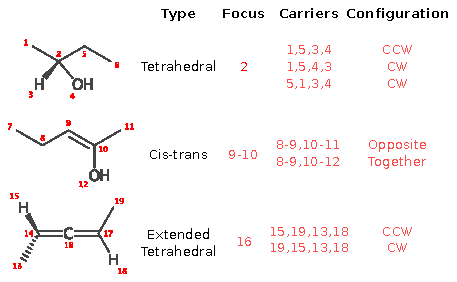
\includegraphics{img/stereodesc_annotated.pdf}

\subsection*{Figure 3 - The raw input files of CHEMBL23970 and CHEMBL444314 are displayed (ChEMBL 21).}\label{fig:stereoprojections}
Without perceiving the stereochemistry indicated by Haworth projection in CHEMBL23970, the database entries are inncorectly considered distinct. Down stream aggregation databases mirror this separation (PubChem CID 5280, CID 65119).

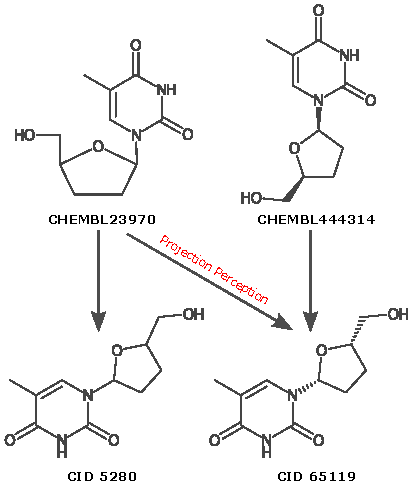
\includegraphics{img/projections_annotated.pdf}

\subsection*{Figure 4 - Integrated example showing the rendering and SMILES
parsing functionality.}\label{fig:depiction}

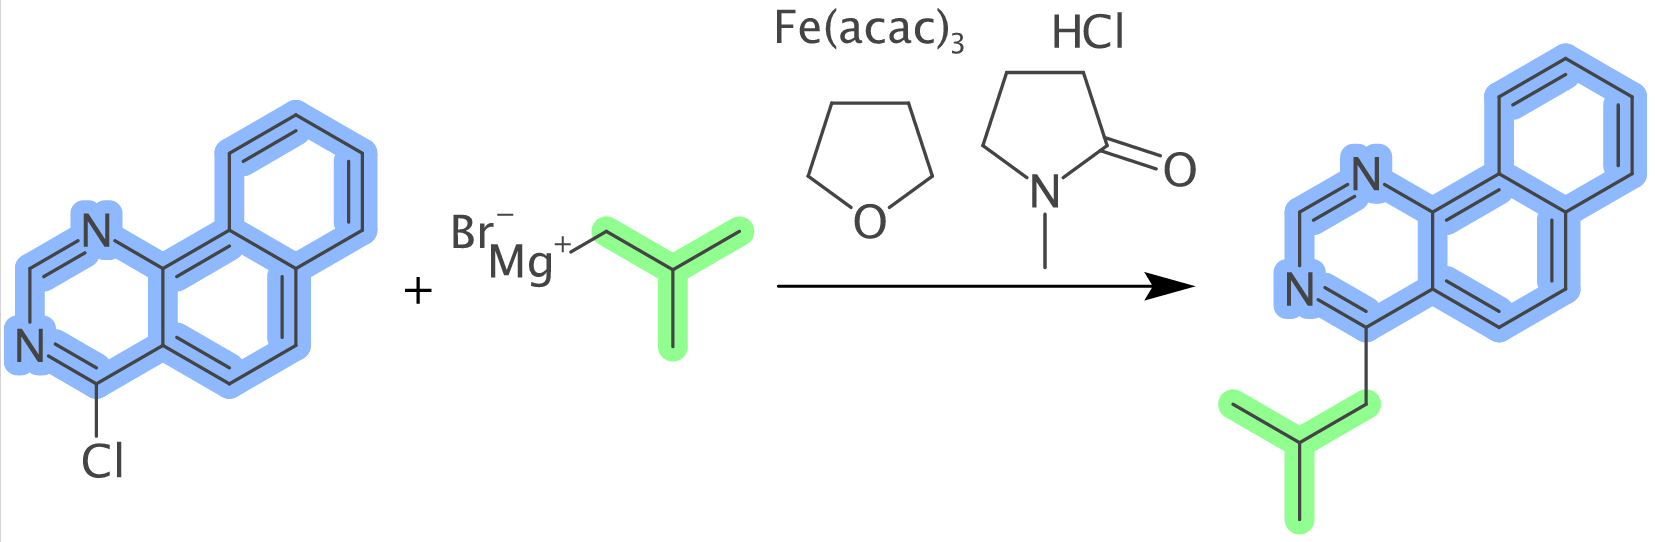
\includegraphics[width=\textwidth]{reaction.png}

\subsection*{Figure 5 - The improved structure diagram generation has improved
code to solve overlap.}\label{fig:sdg}
The original SDG code used general heuristics (left) and the
OverlapResolver would fine tune the layout to ensure atoms would not be placed
at the same location (middle). The new SDG algorithm is able to
make more rigorous changes, making the final output must more pleasing
(right).

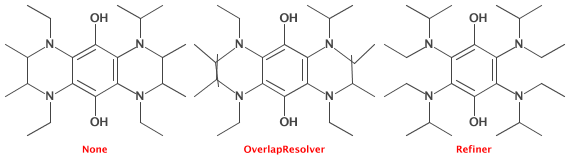
\includegraphics[width=\textwidth]{sdg.png}

  \subsection*{Figure 6 - Dependencies between CDK modules.}\label{fig:deps}
      Visualization of the dependencies between CDK modules. For example,
      the cdk-core depends on the cdk-interfaces module. A few higher level
      modules have been left out: cdk-builder3dtools, cdk-legacy, and
      cdk-depict.

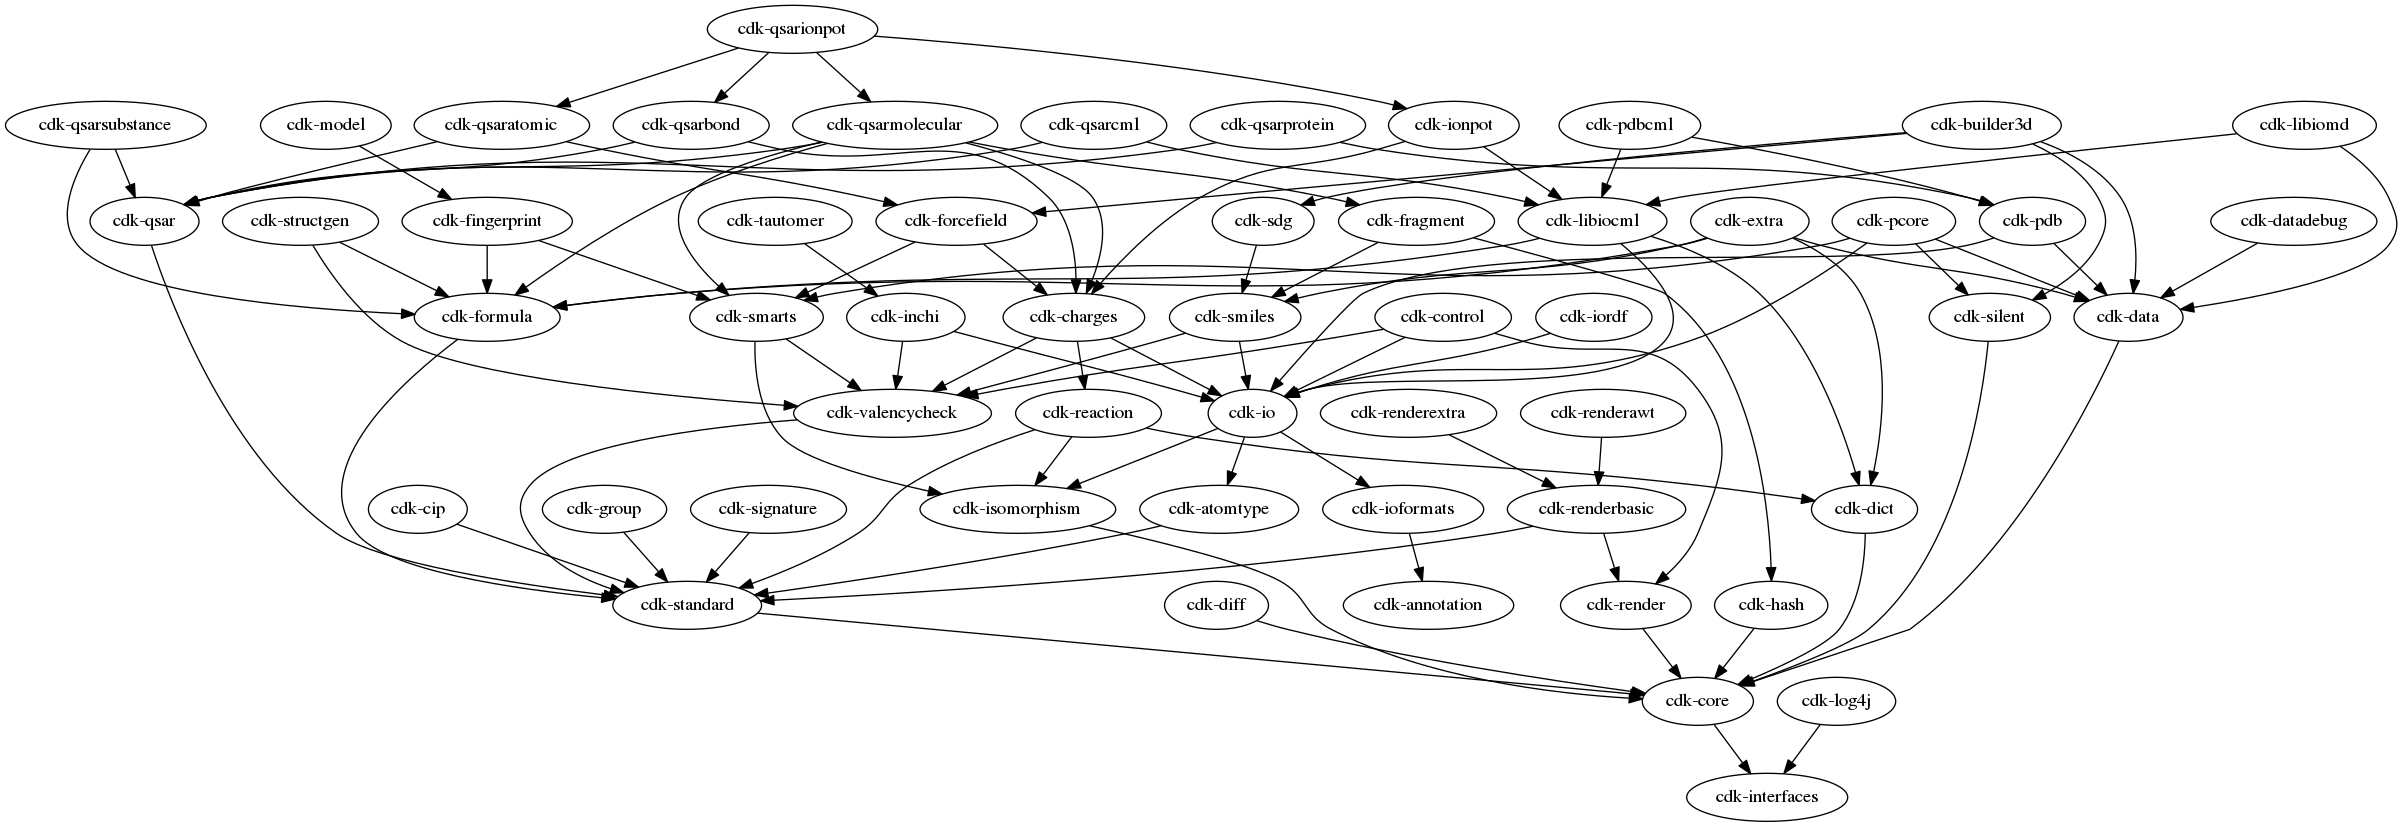
\includegraphics[width=\textwidth]{cdkDeps.png}


\newpage

%%%%%%%%%%%%%%%%%%%%%%%%%%%%%%%%%%%
%% Tables                        %%

\newpage

%% Use of \listoftables is discouraged.
%%
\section*{Tables}


  \subsection*{Table 1 - Evaluation of molecular formula generators.}
  \label{tab:formula_generators}
  The resulting formula counts and runtimes of the HR2, PFG, and CDK chemical
formula generators based on input mass and mass tolerance values. Formulas were
generated using chemical elements C,H,N,O,P,S without bounds (the allowed atom
count was set to 0--10000 for each element). All heuristic filtering rules were
disabled for the purpose of the evaluation. The slight differences in the
number of generated formulas were caused by different isotope masses embedded
in each software and/or by rounding errors during calculation. The runtimes are
average values from three independent runs performed on three different 16-core
Intel Xeon 2.2~GHz CPU workstations equipped with 128~GB RAM, running Ubuntu
Linux version 12.04.5 LTS and OpenJDK Java runtime version 1.7.0\_101.
  \vskip 1\baselineskip

    \begin{minipage}{1\textwidth}
    \centering
    \begin{tabular}{llllllll}
	\multirow{2}{*}{ Mass (Da) } & \multirow{2}{*}{ Tolerance ($\pm$ Da) } & \multicolumn{3}{c}{ \# of generated formulas } & \multicolumn{3}{c}{ Runtime (s) } \\
	& & HR2 & PFG & CDK & HR2 & PFG & CDK \\
	$100$ & $0.001$ & $1$ & $1$ & $1$ & $0.10$ & $\mathbf{0.06}$ & $0.49$ \\
	$100$ & $0.01$ & $18$ & $18$ & $18$ & $0.03$ & $\mathbf{0.01}$ & $0.52$ \\
	$500$ & $0.001$ & $430$ & $430$ & $430$ & $0.51$ & $\mathbf{0.09}$ & $0.67$ \\
	$500$ & $0.01$ & $4\,265$ & $4\,265$ & $4\,264$ & $0.55$ & $\mathbf{0.39}$ & $0.96$ \\
	$1\,000$ & $0.001$ & $8\,572$ & $8\,572$ & $8\,568$ & $16.5$ & $1.5$ & $\mathbf{1.2}$ \\
	$1\,000$ & $0.01$ & $85\,542$ & $85\,542$ & $85\,537$ & $16.8$ & $5.4$ & $\mathbf{3.7}$ \\
	$2\,000$ & $0.001$ & $226\,346$ & $226\,346$ & $226\,323$ & $1156.5$ & $58.9$ & $\mathbf{8.6}$ \\
	$2\,000$ & $0.01$ & $2\,263\,410$ & $2\,263\,410$ & $2\,263\,409$ & $932.5$ & $156.3$ & $\mathbf{69.7}$ \\
	$3\,000$ & $0.001$ & $1\,647\,132$ & $1\,647\,132$ & $1\,647\,118$ & $9\,667.9$ & $603.5$ & $\mathbf{59.3}$ \\
	$3\,000$ & $0.01$ & $16\,471\,338$ & $16\,471\,338$ & $16\,471\,373$ & $9\,694.5$ & $1\,303.6$ & $\mathbf{505.7}$ \\
    \end{tabular}
    \end{minipage}


  \subsection*{Table 2 - The molecular fingerprints in CDK.}
  \label{tab:fingerprints}
  Listed are the currently available molecular fingerprint in CDK with
  information about whether they come as bit / count versions, what CDK version
  they appeared in, their default size and where applicable also relevant
  references.
  \vskip 1\baselineskip

    \begin{minipage}{1\textwidth}
    \renewcommand*{\thempfootnote}{\fnsymbol{mpfootnote}}
    \centering
    \begin{tabular}{lcclc}
                             & Bit version  & Count version & CDK version & Default Size    \\
  CircularFingerprinter~\cite{rogers2010extended, Clark2014}      & $\checkmark$ & $\checkmark$  & 1.6.0 ?     & $1\,024$ / $2^{32}$%
\footnote[1]{For the CirkularFingerprinter the bit version is folded to 1024 whereas the count version is unfolded.} \\
  EStateFingerprinter~\cite{Hall1995}       & $\checkmark$ &               & 1.2.0       & $79$            \\
  ExtendedFingerprinter      & $\checkmark$ &               & 1.0         & $1\,024$        \\
  Fingerprinter              & $\checkmark$ &               & 1.0         & $1\,024$        \\
  GraphOnlyFingerprinter     & $\checkmark$ &               & 1.0         & $1\,024$        \\
  HybridizationFingerprinter & $\checkmark$ &               & 1.4.0       & $1\,024$        \\
  KlekotaRothFingerprinter~\cite{Klekota2008}   & $\checkmark$ &               & 1.4.6       & $4\,860$        \\
  LingoFingerprinter~\cite{vidal2005lingo}         & $\checkmark$ &               & 1.6.0 ?     & NA%
\footnote[2]{The Lingofingerprinter does not have a default size.}
                                                                                             \\
  MACCSFingerprinter         & $\checkmark$ &               & 1.2.0       & $166$           \\
  PubchemFingerprinter~\cite{pubchemFP}       & $\checkmark$ &               & 1.4.0       & $881$            \\
  ShortestPathFingerprinter  & $\checkmark$ &               & 1.6.0 ?     & $1\,024$        \\
  SignatureFingerprinter~\cite{signaturefingerprints}     & $\checkmark$ & $\checkmark$  & 1.6.0 ?     & $2^{32}$         \\
  SubstructureFingerprinter  & $\checkmark$ &               & 1.0         & $307$           \\

    \end{tabular}
    \end{minipage}

      \subsection*{Table 3 - A selection of key CDK modules with major changes.}\label{tab:modules}
  An overview of a selection of often used CDK modules with description,
  dependencies on third-party libraries, and the major changes since
  version~1.2. Dependencies between modules are depicted in Figure~4\ref{fig:deps}.
  \vskip 1\baselineskip

    \begin{minipage}{1\textwidth}
    \renewcommand*{\thempfootnote}{\fnsymbol{mpfootnote}}
    \centering
    \begin{tabular}{lp{3cm}p{3cm}l}
  \textbf{Module}            & \textbf{Description}  & \textbf{Major Changes} & \textbf{Dependencies} \\ \hline
  interfaces                 & Interfaces for the data models. & & Vecmath 1.5.2 \\ \hline
  core                       & Core functionality.             & & Google Guava 17.0 \\ \hline % FIXME: how to add https://github.com/google/guava ?
  standard                   & Common functionality.           & & \\ \hline
  render                     & Graphical rendering.            & Redesigned to make it more modular and support multiple widget toolkits, like AWT and SWT. & \\ \hline
  isomorphism                & Isomorphism and substructure searching. & & \\ \hline
  atomtype                   & Various non-core atom type schemes.     & Unified approach where atom typing is separated from other algorithms. & \\ \hline
  ioformats                  & Definitions of (chemical) input/output formats. & & \\ \hline
  io                         & Readers and writers for input/output formats.  & The MDL molfile reader has been rewritten and supports in atom types defind in the specification. & XPP3 1.1.4c \\ \hline
  iordf                      & Stores data models as in the Resource Description Framework serialization foramts. & New. & Jena 2.7.4 \\ \hline
  inchi                      & IUPAC International Chemical Identifier support. & & JNI-InChI 0.8~\cite{Spjuth2013}  \\ \hline
  libiocml                   & Writer for the Chemical Markup Language format. & & XOM 1.2.5, CMLXOM 3.1~\cite{Murray-Rust2011} \\ \hline
  sdg                        & Structure diagram generation.  & Much improved overlap resolution. & \\ \hline
  smiles                     & Reading and writing in the SMILES format. & SMILES support performance and converage is greatly improved. & Beam 0.9.1~\cite{Beam} \\ \hline
  smarts                     & Substructure searching with the SMARTS format. & & Beam 0.9.1~\cite{Beam} \\ \hline
  formula                    & Chemical formula support. & New. & \\ \hline
  fingerprint                & Calculate fingerprints. & Many new fingerprint types (see text). & Apache Commons Math 3.1.1 \\ \hline
  qsar and qsarmolecular                       & Molecular descriptors.  & & XOM 1.2.5, JAMA 1.0.3~\cite{Hicklin2012} \\ \hline
  signatures                 & Calculation of molecular and atomic signatures. & & Signatures 1.1 \\ \hline % FIXME: ask Gilleain for the reference
    \end{tabular}
    \end{minipage}


\end{backmatter}

\end{document}







